\documentclass[12pt]{article}
\usepackage[top=1in,bottom=1in,left=1in,right=1in]{geometry}
\usepackage{alltt}
\usepackage{array}	
\usepackage{graphicx}
\usepackage{tabularx}
\usepackage{verbatim}
\usepackage{setspace}
\usepackage{listings}
\usepackage{amssymb,amsmath, amsthm}
\usepackage{qtree}
\usepackage{hyperref}
\usepackage{oz}
\usepackage[cc]{titlepic}
\usepackage{fancyvrb}
\usepackage{epstopdf}
\usepackage{soul}
\graphicspath{ {./figures/} }

\newcolumntype{L}{>{\centering\arraybackslash}m{3cm}}

\title{Concordia University\\
Department of Computer Science and Software Engineering\\
\textbf{SOEN 331 - S\\Formal Methods for Software Engineering}\\
\ \\
\textbf{Assignment 1: Fundamentals}}
\author{\textbf{Witnick-Hans Joseph}\\
		\texttt{ID: 29348743}\\
		\textbf{Alexandra Zana}\\
		\texttt{ID: 40131077}\\
		\textbf{Alexandre Eid}\\
		\texttt{ID: 40155833}
\ \\}
\date{October 14, 2021.}

\begin{spacing}{1.5}
\begin{document}
\maketitle

\newpage
\tableofcontents
\newpage

\section{General information}

\noindent \textbf{Date posted}: Thursday 30 September, 2021.\\
\noindent \textbf{Date due}: Thursday, 14 October, 2021, by 23:59.\\
\noindent \textbf{Weight}: 15\% of the overall grade.

\section{Introduction}
You should form a team of \textbf{three} members. Each team should designate a leader who will submit the assignment electronically. In case you cannot find a team, please contact me and I will assign you to one. There are \textbf{7} problems in this assignment, with a total weight of \textbf{100} points. You must prepare all your solutions in~\LaTeX~and produce a single \texttt{pdf} file. Name the file after the Concordia id of the person who will submit, e.g. \texttt{123456.pdf}.\\

\section{Ground rules}

This is an assessment exercise.  You may not seek any assistance while expecting to receive credit. \textbf{You must work strictly within your team and seek no assistance for this assignment ((e.g. from the teaching assistants, fellow classmates and other teams or external help)}. Please note that you should \textbf{not} discuss the assignment during tutorials. I am available to discuss clarifications in case you need any.\\

\noindent \textbf{All team members are expected to work relatively equally on each problem}. The team leader has the responsibility to ensure that the team does not violate this rule. \textbf{In your submission, you must include only the names of those team members who contributed to the assignment.} Accommodating someone who did not contribute will result in a penalty.\\

\noindent If there is any problem in the team (such as lack of contribution, etc.), the team leader must contact the instructor as soon as the problem appears.

\newpage

\section{Problems}

\subsection{Propositional logic (10 pts)}

\noindent You are shown a set of four cards placed on a table, each of which has a \textbf{letter} on one side and a \textbf{symbol} on the other side. The visible faces of the cards show the letters \textbf{L} and \textbf{A}, and the symbols \textbf{$\Box$}, and \textbf{$\diamondsuit$}.\\

\noindent Which card(s) must you turn over in order to test the truth of the proposition that \textit{``If a card has a consonant on one side, then it has the symbol $\diamondsuit$ on the other side''}? Explain your reasoning \underline{in detail} by deciding for \underline{each} card whether it should be turned over and why. In your answers, apply any and all appropriate validating or non-validating patterns where applicable.\\


\subsubsection{Propositional logic answer}

\noindent We have two statements:

\indent p: The card has a consonant

\indent q: The card has symbol \textbf{$\diamondsuit$}

$ p \rightarrow q$ , $ \neg q \rightarrow \neg p$
\begin{itemize}
	\item Card \textbf{$\diamondsuit$}: Implication does not necessarily entail causation. So even if the card is a \textbf{$\diamondsuit$} the othe side value could be L or A. It is not the card to turn.

	\item Card \textbf{$\square$}: Since this card is a vowel, we can check the validity of the contrapositive $ \neg q \rightarrow \neg p$. This should be a card to turn. This card does not satisfy the second statement that the card is a \textbf{$\diamondsuit$}. So we cannot evaluate the second statement. It is not the card to turn.
	
	\item Card L: Since this card is a consonant, we can check the validity of $ p \rightarrow q$. We can check the back to validate q. This should be a card to turn.
	
	\item Card A: This card is like $ \neg p $, "A" is not a consonent, and therefore does not help in showing $ p \rightarrow q$ or $ \neg q \rightarrow \neg p$
	
\end{itemize}

\newpage

\subsection{Predicate logic 1 (10 pts)}

In the domain of all people, consider the predicate \textit{disclosed(a, b)} that is interpreted as \textit{``a has disclosed a secret to  b.''}
\begin{enumerate}
\item How are the following two expressions translated into plain English? Are the two expressions logically equivalent?
\begin{itemize}
	\item $\forall a \exists b~disclosed(a, b)$.
	\item $\exists b \forall a ~disclosed(a, b)$.
\end{itemize} 
\item Can we claim that $\forall a \exists b~disclosed(a, b) \rightarrow \exists b \forall a ~disclosed(a, b)$? Discuss in detail.
\item Can we claim that $\exists b \forall a ~disclosed(a, b) \rightarrow \forall a \exists b~disclosed(a, b)$? Discuss in detail.
\end{enumerate}

\subsubsection{Problem 2 answer}
\begin{enumerate}
\item translation
	\subitem $\forall a \exists b~disclosed(a, b)$: Everyone has disclosed a secret to someone. 
	\subitem $\exists b \forall a ~disclosed(a, b)$: There exists someone who has been disclosed a secret by everyone.
	The two expression are not logically equivalent. Here is a proof by counter example using diagrams. We can see that they are not the same
	\begin{center}
	\begin{tabular}{cc}
		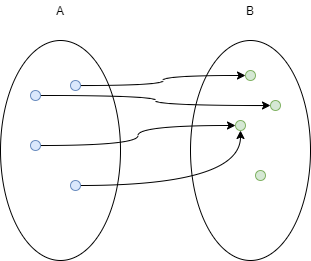
\includegraphics[scale=0.5] {all-a-told-some-b.png}  &
		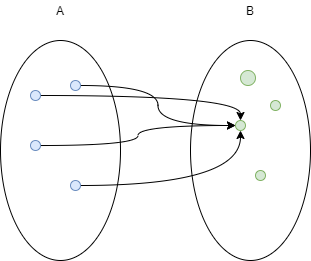
\includegraphics[scale=0.5] {some-b-has-been-told-by-all-a}\\
		$\forall a \exists b~disclosed(a, b)$ &
		$\exists b \forall a ~disclosed(a, b)$\\
	\end{tabular}
	\end{center}

\item We cannot claim that $\forall a \exists b~disclosed(a, b) \rightarrow \exists b \forall a ~disclosed(a, b)$.\\
	In the first statement, we are saying that everyone has disclosed a secret to someone, and thethe other is saying someone has been told be everyone a secret.\\
	The first statement implies that the person $b$ might not be the same person for each person $a$. \\
	The second statement implies that every $a$ has told a secret to the same $b$.

	\subitem  
\item Yes, we can claim that $\exists b \forall a ~disclosed(a, b) \rightarrow \forall a \exists b~disclosed(a, b)$.\\
 if at least one $b$ has been disclosed a secret by all the $a$'s,\\ 
 then we can safely say that all the $a$ have disclosed a secret to a $b$.
\end{enumerate} 


\newpage

\subsection{Predicate logic 2 (10 pts)}

\noindent Consider the subject ``x is a person'' and the predicate ``x is a mortal'', together with the following list of categorical propositions:
\begin{itemize}
\item ``No person is immortal.''

\item ``All people is immortal.''

\item ``Some people are mortal.''	

\item ``Some people are not mortal.''	
\end{itemize} 


\begin{enumerate}
\item  ``Identify each categorical statement with its name (i.e. letter description)''.
\subitem answer:
\subitem "No person is immortal.": A Form
\subitem "All people are immortal.": E Form
\subitem "Some people are mortal.": I Form
\subitem "Some people are not mortal.": O Form 

\item ``Identify universal statements.''
\subitem answer: 
\subitem "No person is immortal." and "All people are immortal."

\item ``Identify particular statements.''
\subitem answer:
\subitem "Some people are mortal." and "Some people are not mortal."

\item ``Identify affirmative statements''
\subitem answer:
\subitem "No person is immortal." and "Some people are mortal."

\item ``Identify negative statements.''
\subitem answer: 
\subitem "All people are immortal." and "Some people are not mortal."

\item ``Identify statements with opposite truth values''
\subitem answer:  

\item ``Identify statements that cannot both be true, but could both be false.''
\subitem answer:  

\item ``Identify statements that cannot both be false but could both be true.''
\subitem answer:  

\item ``Identify pairs of super-subaltern statements.''
\subitem answer:  

\end{enumerate}


\newpage

\subsection{Ordered structures (10 pts)}

Consider a list $\Lambda = \langle w, x, y, z \rangle$, deployed to implement a stack Abstract Data Type.

\begin{enumerate}

\item Let the head of $\Lambda$ correspond to the topmost position of the Stack. Implement the body of operations \texttt{push(el, $\Lambda$)} and \texttt{pop($\Lambda$)} (let return element be held in variable topmost) using list construction operations. In both cases a)  we assume that appropriate preconditions exist, and b) we can refer to $\Lambda'$ as the state of the list upon successful termination of one of its operations.

\noindent answer: 

\indent \texttt{push(el, $\Lambda$)}  can be written as $\Lambda' = cons( el, \Lambda) = \langle el, w, x, y, z \rangle$.


\indent \texttt{pop($\Lambda$)}  can be written as $head(\Lambda) = element = w$ and $\Lambda' = tail(\Lambda) = \langle x, y, z \rangle$,

\item  Let the last element of $\Lambda$ correspond to the topmost position of the Stack. Implement the body of both operations as above. When applicable, use control flow statements in your answer.

\end{enumerate}

\newpage

\subsection{Unordered structures and type declarations (10 pts)}
Consider the sets
\begin{itemize}
	\item Laptop = \{Apple,IBM , Sony, HP, Acer , Dell, LG\}, and
	\item Favorite = \{Apple, Sony, Dell\}.
\end{itemize}
Answer the following questions:
\begin{enumerate}
	\item How do we interpret the expression Favorite : $\mathbb{P}$Laptop?
	\subitem answer: 
	\subitem The variable Favorite can assume any value supported by $\mathbb{P}$Laptop (ie: the var Favorite can be any value of the PowerSet of Laptop)
	\item Is $\mathbb{P}$Laptop a legitimate type?
	\subitem answer: 
	\subitem Yes; Favorite is of type $\mathbb{P}$Laptop. The powerset Laptop is a legitimate type.
	\item What is the nature of the variable in Favorite : $\mathbb{P}$Laptop? (i.e. Atomic or composite? If composite, what type?)
	\subitem answer: 
	\subitem It is a composition. the variabale Favorite: $\mathbb{P}$Laptop is a set of elements, so it is a composition.
	\item Is Apple $\in \mathbb{P}$Laptop? Explain why or why no
	\subitem answer:
	\subitem No; the $\mathbb{P}$Laptop is a list of all possible subsets we can produce from the set Laptop, and the atomic element Apple is not an element of $\mathbb{P}$Laptop.
	\item Is \{Apple\} $\in \mathbb{P}$Laptop? Explain why or why not.
	\subitem answer:
	\subitem Yes; since \{Apple\} is a valid element of the $\mathbb{P}$Laptop set. The list element of any atomic element is within the PowerSet of its type.
	\item Is \{\{\}\} $\in \mathbb{P}$Laptop?
	\subitem answer:
	\subitem No, because list Laptop itself does not contain the empty element \{\}, it's power set can't contain the element \{\{\}\}.
	\item Is \{\} $\in \mathbb{P}$Laptop? Explain why or why not.
	\subitem answer:
	\subitem Yes; since the null/empty element is an element of any power set.
	\item If we define variable Favorite : $\mathbb{P}$Laptop, is \{\} a legitimate value for variable Favorite? Explain why or why not.
	\subitem answer:
	\subitem Yes, because the $\mathbb{P}$Laptop contains the empty list element. Ie, if we remove all the elements contained in Favorite, we will have \{\} set.
	\item Is Favorite $\in \mathbb{P}$Laptop? Explain.
	\subitem answer:
	\subitem Yes; the elements of Favorite are elements in $\mathbb{P}$Laptop, but the variable Favorite itself is not.
	\item Is Favorite $\subset \mathbb{P}$Laptop? Explain.
	\subitem answer:
	\subitem No
\end{enumerate}
\newpage

\subsection{Relational calculus 1 (25 pts)}
Consider a system that assigns id’s to locations. An id may represent a vehicle in a parking
lot, a train in a station, a process in an operating system etc. A location may represent a
parking spot, a train station platform, a core in a hardware system etc. The requirements
of the system are as follows:
\begin{enumerate}
	\item Id’s are unique.
	\item An id is assigned to a single location (and maybe re-assigned subsequently).
	\item No multiple id’s may be assigned to the same location.
\end{enumerate}
The model of the system is captured by a relation assignment, which is represented as a set
as shown below:
\[
assignment = \\
\{ \\
\hspace{10mm} 001 \mapsto A,\\
\hspace{10mm} 002 \mapsto B,\\
\hspace{10mm} 003 \mapsto C\\
\}
\]

\begin{enumerate}
	\item Define the precondition to operation add, that assigns a new id to a location.
	\item Provide two alternative definitions for the main functionality of the operation.
	\item What would be the result of calling the operation with id? = 001, and location? = D?
	\item Let us get rid of the precondition. What would be the result of calling add with\\ id? = 004, and location? = C? Would you accept or reject the call? If accepted then the pair should be added to the relation. If rejected, it should not be added to the relation.
	\item Assume that in the absence of a precondition, we attempted to call operation add with some input parameters id? and location?. Under what conditions, if any, would this be acceptable?
	\item Consider operation reassign that modifies the location of an existing id. Define the precondition to operation reassign.
	\item Define the body of operation reassign.
\end{enumerate}
\newpage

\subsection{Relational calculus 2 (25 pts)}
Consider the following relation:

\[ cellphones : Model \leftrightarrow Brand \]

\noindent where

\[
cellphones = \\
\{ \\
\hspace{10mm} galaxyA21s \mapsto samsung,\\
\hspace{10mm} mate10 \mapsto huawei,\\
\hspace{10mm} mate10pro \mapsto huawei,\\
\hspace{10mm} galaxyA01 \mapsto samsung,\\
\hspace{10mm} iPhone12ProMax \mapsto apple,\\
\hspace{10mm} iPhoneSE \mapsto apple,\\
\hspace{10mm} galaxyJ2Core \mapsto samsung,\\
\hspace{10mm} redmi6A \mapsto xiaomi,\\
\hspace{10mm} redmi8 \mapsto xiaomi\\
\}
\]
\begin{enumerate}
	\item Given the above relation,
	\begin{enumerate}
		\item Define the domain of cellphones.\\
		answer: \\
		\indent domain cellphones = Model = \{galaxyA21s, mate10, mate10pro, galaxyA01, iPhone12ProMax, iPhoneSE, galaxyJ2Core, redmi6A, redmi8\}		
		\item Define the range of cellphones.\\
		answer: \\
		range cellphones = Brand = \{samsung, huawei, apple, xiaomi\}
	\end{enumerate}

	\item Given the following the expression:\\ \{galaxyA01, galaxyJ2Core, redmi8\} $\lhd$ cellphones
	\begin{enumerate}
		\item What is the meaning of operator $\lhd$? \\
			answer: $\vartriangleleft$ is a domain restriction, it selects pairs according to the first element.
		\item What is the value of the expression?	\\
		\indent answer: \\ 
		\indent \{galaxyA01, galaxyJ2Core, redmi8\} $\vartriangleleft$ cellphones = \{ \\
		galaxyA01 $\mapsto$ samsung, \\ 
		galaxyJ2Core $\mapsto$ samsung, \\
		redmi8 $\mapsto$ xiaomi \\ 	
		\}
		\item Where would you deploy the operator $\lhd$ in the context of a database management system?\\
		answer: This operator is used to model database queries.
	\end{enumerate}

	\item Given the following the expression:\\ cellphones $\rhd$ \{samsung, xiaomi\}
	\begin{enumerate} 
		\item What is the meaning of operator $\rhd$? \\
		answer: 
		$\rhd$ is a range restriction operator; It assignes pairs based on the second element.
		\item What is the value of the expression?
		cellphones $\rhd$ \{samsung, xiaomi\} = \\
		\{ \\
		galaxyA21s $\mapsto$ samsung, \\
		galaxyA01 $\mapsto$ samsung, \\
		galaxyJ2Core $\mapsto$ samsung, \\
		redmi6A $\mapsto$ xiaomi,\\
		redmi8 $\mapsto$ xiaomi
		\item Where would you deploy such operator in the context of a database management system? \\ 
		answer: \\ 
		This operator is used to model database queries.
	\end{enumerate}

	\item Given the following the expression:\\ \{mate10pro, iPhoneSE, galaxyJ2Core\} $\ndres$ cellphones 
	\begin{enumerate} 
		\item What is the meaning of operator $\ndres$?\\
		answer:\\ 
		It is a domain subtraction, it removes all specified element from the domain of the relation.
		\item What is the value of the expression?	\\
		answer:\\
		\indent cellphones' = \{mate10pro, iphoneSE, galaxyJ2Core\}  $\ndres$ cellphones = \{ \\
		galaxyA21s $\mapsto$ samsung,\\
		mate10 $\mapsto$ huawei,\\
		galaxyA01 $\mapsto$ samsung,\\
		iphone12ProMax $\mapsto$ apple,\\
		redmi6A $\mapsto$ xiaomi,\\
		redmi8 $\mapsto$ xiaomi\\
		\}
		\item Where would you deploy such operator in the context of a database management system?\\
		answer:\\
		This operator would be deployed when we want to delete elements from the database.
	\end{enumerate}

	\item Given the following the expression:\\ cellphones $\nrres$ \{apple, xiaomi\}
	\begin{enumerate} 
		\item What is the meaning of operator $\nrres$?\\
		answer:\\
		$\nrres$ is a range subtraction operator, it removes all elements from the range of the relation.
		\item What is the value of the expression?\\
		answer:\\	
		cellphones' = cellphones $\nrres$ \{apple, xiaomi\} = \{\\
		galaxyA21s $\mapsto$ samsung,\\
		mate10 $\mapsto$ huawei,\\
		mate10pro $\mapsto$ huawei,\\
		galaxyA01 $\mapsto$ samsung,\\
		galaxyJ2Core $\mapsto$ samsung,\\
		\}
		\item Where would you deploy such operator in the context of a database management system?\\
		answer:\\
		You would use $\nrres$ when wanting to modify the content of a database (deleting element, in the case of $\nrres$).
	\end{enumerate}
	
	\item Given the following the expression:\\ cellphones $\oplus$ \{galaxyA51 7→ samsung, mate9 7→ huawei\}
	\begin{enumerate} 
		\item What is the meaning of operator $\oplus$? \\
		\indent answer: \\
		\indent $\oplus$ is a relational overide

		\item What is the value of the expression?	\\
		answer: \\ 
		\indent cellphones $\oplus$ \{galaxyA51 $\mapsto$ samsung, mate9 $\mapsto$ huawei\} = \{ \\ 
		galaxyA21s $\mapsto$ samsung,\\
		mate10 $\mapsto$ huawei,\\
		mate10pro $\mapsto$ huawei,\\
		galaxyA01 $\mapsto$ samsung,\\
		iphone12ProMax $\mapsto$ apple,\\
		iphoneSE $\mapsto$ apple,\\
		galaxyJ2Core $\mapsto$ samsung,\\
		redmi6A $\mapsto$ xiaomi,\\
		redmi8 $\mapsto$ xiaomi,\\
		galaxyA51 $\mapsto$ samsung,\\
		mate9 $\mapsto$ huawei,\\
		\}

		\item Where would you deploy such operator in the context of a database management system?\\
		\indent answer: \\
		\indent This operator would be used in the event that we want to add or modify elements in the database.

		\item  Does the result of the expression have a permanent effect on the database (relation)? If not, describe in detail how would you ensure that such operation would have a permanent effect.\\
		\indent answer:\\
		\indent The expression doesn't have a permanent effect. If we want to have a permanent effect, we would need to have an assignment operation as such:\\
		\indent cellphones' = cellphones $\oplus$ \{galaxyA51 $\mapsto$ samsung, mate9 $\mapsto$ huawei\}\\
		\indent We need to assign the value of the expression to cellphone to have permanent effect.\\
		
	\end{enumerate}
\end{enumerate}

\newpage

\section{What to submit}

\noindent Please submit your \texttt{pdf} file at the Electronic Assignment Submission portal

\centerline{(\url{https://fis.encs.concordia.ca/eas}) }

\noindent under \textbf{Theory Assignment 1}.

\end{spacing}

\end{document}